\documentclass{article}

\usepackage[margin=0.5in,bottom=1in]{geometry}

\usepackage{amsmath}

\usepackage{multicol}
\setlength{\columnsep}{1cm}

\usepackage{lipsum}% for dummy text
\usepackage[varg]{txfonts}
\usepackage{graphicx}
\usepackage{subcaption}
\usepackage{multirow}

\usepackage{titlesec}
\titleformat{\section}{\fontfamily{phv}\fontsize{12}{15}\bfseries}{\thesection}{1em}{}
\titleformat{\subsection}{\fontfamily{phv}\fontsize{10}{15}\itshape}{\thesubsection}{1em}{}

\title{\textbf{FYS4150 Project 1: \\1-dimensional Poisson equation}}
\author{Marie Foss, Maria Hammerstr{{\o}}m}
\date{} % removes date from title

\begin{document}

\maketitle

\begin{abstract}
	\noindent \lipsum[1] 
	\vspace*{2ex}
\end{abstract}



\begin{multicols}{2}

\section{Introduction}
In this project we will solve the one-dimensional Poissson equation with Dirichlet boundary conditions by rewriting it as a set of linear equations and solving these numerically in a program written in C++.The equation to be solved is:

\begin{equation}\label{eq:Poisson}
	-u''(x) = f(x) \hspace{0.5cm} x\in(0,1), \hspace{0.5cm} u(0) = u(1) = 0
\end{equation}

\noindent and we define the discretized approximation  to $u$ as $v_i$  with grid points $x_i=ih$   in the interval from $x_0=0$ to $x_{n+1}=1$. The step length or spacing is defined as $h=1/(n+1)$. We then have the boundary conditions $v_0 = v_{n+1} = 0$. We can approximate the second derivative of $u$ with:

\begin{equation}\label{eq:second_derivative}
   -\frac{v_{i+1}+v_{i-1}-2v_i}{h^2} = f_i  \hspace{0.5cm} \mathrm{for} \hspace{0.1cm} i=1,\dots, n,
\end{equation}

\noindent where $f_i=f(x_i)$. Eq. (\ref{eq:second_derivative}) can be written as a linear set of equations of the form: 

\begin{equation}
	{\bf A}{\bf v} = \tilde{{\bf b}}
\end{equation}

\noindent where $\tilde{b}_i=h^2f_i$ and \textbf{A} is an $n\times n$ matrix of the form:

\begin{equation}
    {\bf A} = \left(\begin{array}{cccccc}
                           2& -1& 0 &\dots   & \dots &0 \\
                           -1 & 2 & -1 &0 &\dots &\dots \\
                           0&-1 &2 & -1 & 0 & \dots \\
                           & \dots   & \dots &\dots   &\dots & \dots \\
                           0&\dots   &  &-1 &2& -1 \\
                           0&\dots    &  & 0  &-1 & 2 \\
                      \end{array} \right)
\end{equation}

\noindent This can be shown by writing it out. We then get
\begin{align}
	2v_1 - v_2 &= \tilde{b}_1 \\
	-v_1 + 2v_2 - v_3 &= \tilde{b}_2 \\
	-v_2 + 2v_3 - v_4 &= \tilde{b}_3 \\
	... \\
	-v_{i-1} + 2v_n - v_{i+1} &= \tilde{b}_i,
\end{align}
which is the same as Eq. (\ref{eq:second_derivative}). 

We will assume that the source term is $f(x) = 100e^{-10x}$. Using the interval and boundary conditions as stated above, the above differential equation has a closed-form  solution given by $u(x) = 1-(1-e^{-10})x-e^{-10x}$. We will compare our numerical solution with this result. 





\section{Methods}
\subsection{Simple algorithm}
In our case we are dealing with a simple tridiagonal matrix. We can therefore rewrite our matrix \textbf{A} in terms of one-dimensional vectors \textit{a, b, c} of length 1:\textit{n}. The linear equation then reads:

\begin{equation}
    {\bf A} = \left(\begin{array}{cccccc}
                           b_1& c_1 & 0 &\dots   & \dots &\dots \\
                           a_2 & b_2 & c_2 &\dots &\dots &\dots \\
                           & a_3 & b_3 & c_3 & \dots & \dots \\
                           & \dots   & \dots &\dots   &\dots & \dots \\
                           &   &  &a_{n-2}  &b_{n-1}& c_{n-1} \\
                           &    &  &   &a_n & b_n \\
                      \end{array} \right)\left(\begin{array}{c}
                           v_1\\
                           v_2\\
                           \dots \\
                          \dots  \\
                          \dots \\
                           v_n\\
                      \end{array} \right)
  =\left(\begin{array}{c}
                           \tilde{b}_1\\
                           \tilde{b}_2\\
                           \dots \\
                           \dots \\
                          \dots \\
                           \tilde{b}_n\\
                      \end{array} \right).
\end{equation}

\noindent which can be written as:

\begin{equation}\label{eq:tridiagonal_system}
  a_iv_{i-1}+b_iv_i+c_iv_{i+1} = \tilde{b}_i
\end{equation}

\noindent for $i=1,2,\dots,n$. We want to find a simple algorithm to solve this set of equations. To do this, we can rewrite Eq.~\ref{eq:tridiagonal_system} by a method of elimination, which will lead to a system where there is only one unknown. 

The first thing to do is to realize that Eq.~\ref{eq:tridiagonal_system} gives a system of three equations:

\begin{align}
	b_1 v_1 + c_1 v_2 &= \tilde{b}_1, \hspace{0.5cm} i = 1  \\
	a_i v_{i-1} + b_i v_i + c_i v_{i+1} &= \tilde{b}_i, \hspace{0.5cm} i = 2, \dots, n - 1 \\
	a_n v_{n-1} + b_n v_n &= \tilde{b}_n, \hspace{0.5cm} i = n  
\end{align}


\noindent where the boundary conditions have been applied to simplify the equations. The idea now is to subtract one row with a scalar multiple of another to eliminate variables. First we want to eliminate $v_1$:\\

(something)\\

\noindent Then we can follow the same approac to eliminate $v_2$:\\

(something)\\

\noindent The algorithm for solving this equation can be stated as follows:\\

(algorithm)



\subsection{LU decomposition}
In addition to solving the linear second-order differential equation Eq.~\ref{eq:Poisson} using the simple algorithm described above, we want to solve the equation using LU decomposition, then compare the results. For this we will use the provided \verb@lib.cpp@ library.

(More coming here about what LU decomposition is!!)




\section{Results}    \label{sec:analysis}

\subsection{Comparing the analytical and numerical solution}
We can run our code for different values of $n$ and plot the analytical and numerical solution to see how well they correspond. For different values of $n$, see Fig.~\ref{fig:n-values}.

\begin{figure*}
\begin{center}
\begin{tabular}{cc}
  	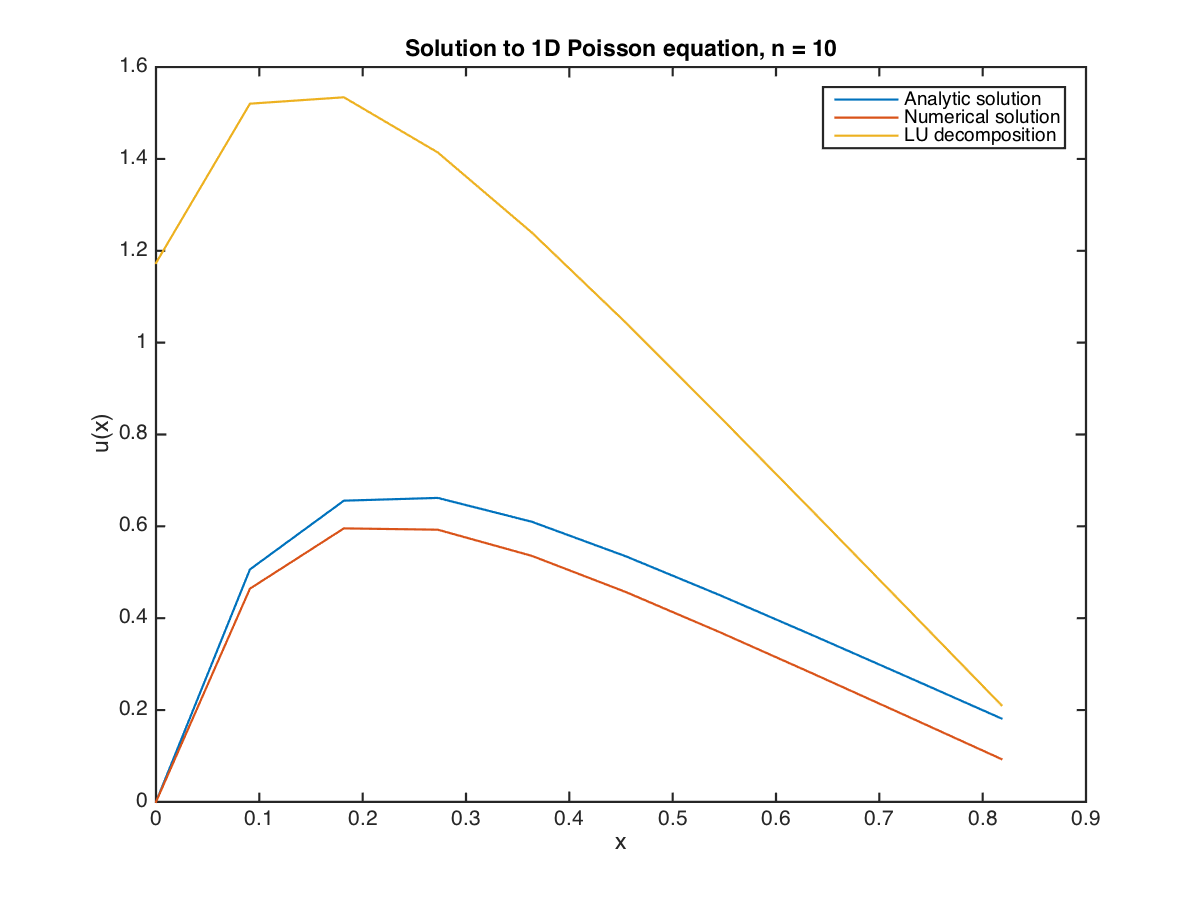
\includegraphics[width=90mm]{../build-Project1-Desktop_Qt_5_5_0_clang_64bit-Debug/Plot_n10.png} 	
	& 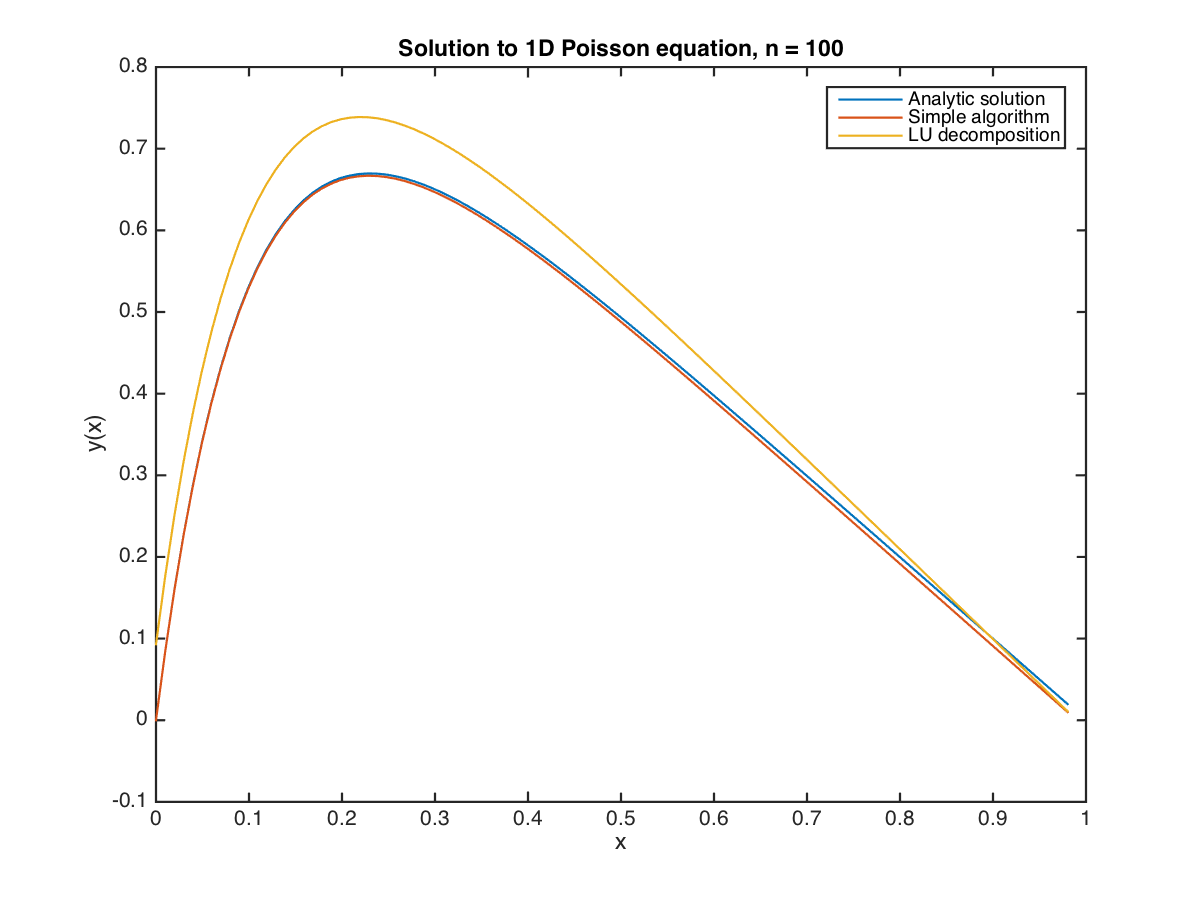
\includegraphics[width=90mm]{../build-Project1-Desktop_Qt_5_5_0_clang_64bit-Debug/Plot_n100.png} \\
	
	(a) $n$ = 10 								& (b) $n$ = 100 \\[6pt]
	
 	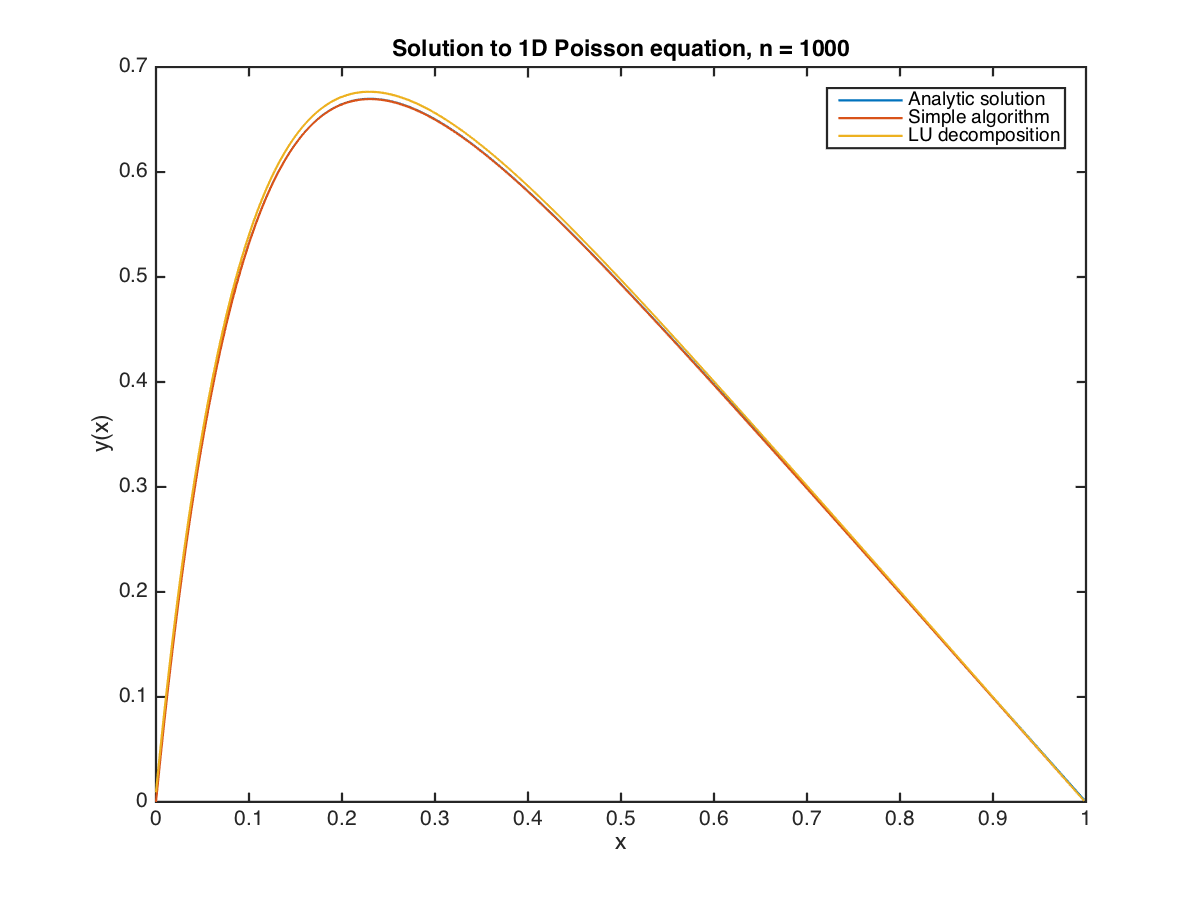
\includegraphics[width=90mm]{../build-Project1-Desktop_Qt_5_5_0_clang_64bit-Debug/Plot_n1000.png} 	
	& 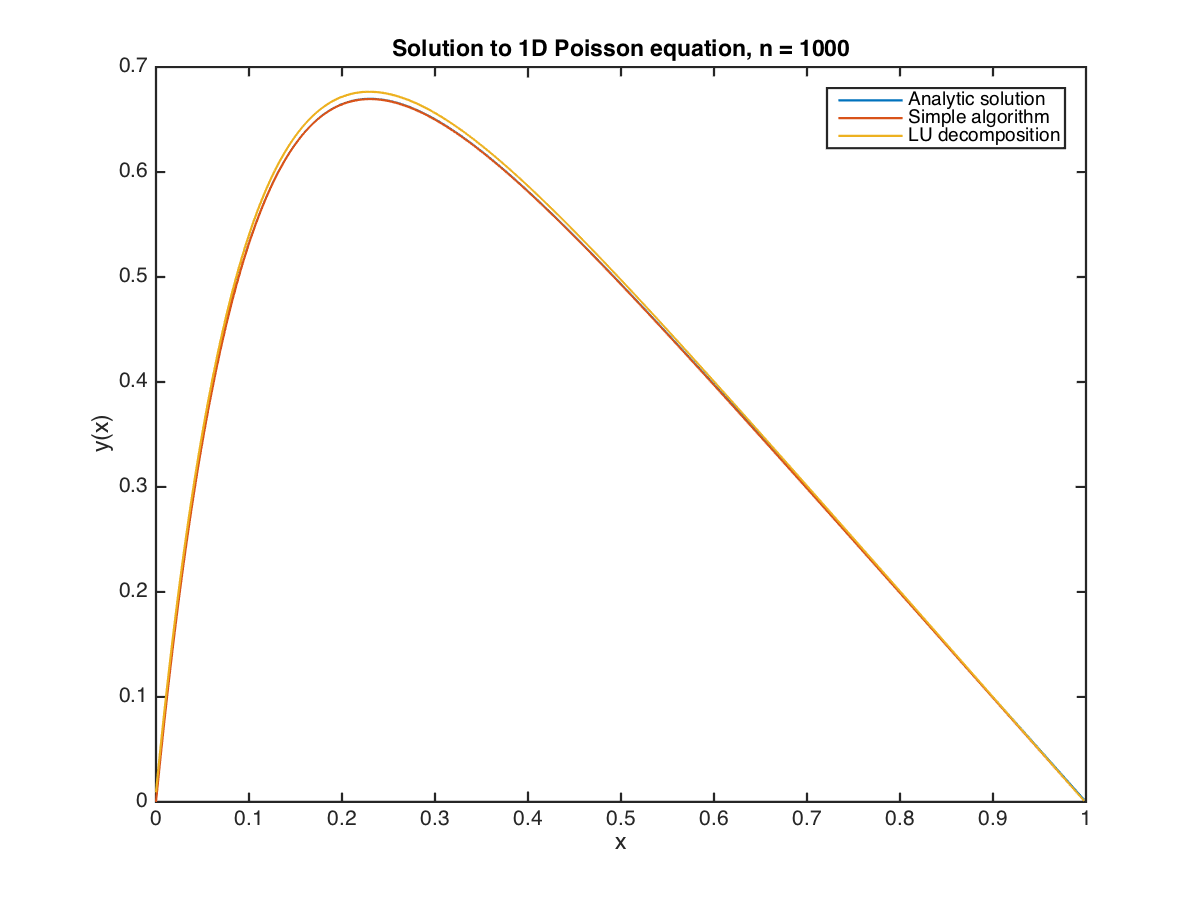
\includegraphics[width=90mm]{../build-Project1-Desktop_Qt_5_5_0_clang_64bit-Debug/Plot_n1000.png} \\
	(c) $n$ = 1 000 								& (d) $n$ = 10 000 (still waiting on program) \\[6pt]
	
\end{tabular}
\caption{Comparison of the three different solutions for different values of $n$.}\label{fig:n-values}
\end{center}
\end{figure*}


\subsection{Relative errors}

The relative error in the data set is computed by calculating:

\begin{equation}
   \epsilon_i=log_{10}\left(\left|\frac{v_i-u_i}
                 {u_i}\right|\right),
\end{equation}

\noindent for $i = 1, \dots, n$ for the function values $u_i$ and $v_i$, where $u_i$ represents the closed-form analytical solution, while $v_i$ is the numerical solution given by the simple algorithm described above. The relative error will be a function of $log_{10}(h)$. For each step length $h$ we want to extract the max value of the relative error. Doing this while increasing $n$ to $n=10000$ and $n=10^5$, gives the following results:

\begin{center}
\begin{tabular}{ l l }\hline
	$n$ 		&Maximum error \\ \hline
	10 		& 1.18895 \\
	100 		& 1.03632 \\
	$10^3$ 	& 1.00786 \\
	$10^4$ 	& 1.00076 \\
	$10^5$ 	&XX\\
	\hline
\end{tabular}
\end{center}

\begin{center}
Table 1: Maximum error as a function of step length.
\end{center}

\subsection{Number of floating point operations and time usage}
Some of the methods described above may be more computationally heavy for a computer to do than others. One way to evaluate this is to calculate the precise number of floating point operations ("FLOPS") needed to solve the equations.

Gaussian elimination requires $\frac{2}{3}n^3 + O(n^2)$ FLOPS and LU decomposition requires $O(n^3)$. By counting the floating point operations in our code, we find that for our tridiagonal system, $8n + 1$ FLOPS are required. 

The number of floating point operations and time usage in the different cases, are shown in the table below.


\begin{center}
    \begin{tabular}{ l  l  l  l } \hline
    \textbf{Method} 					&\textbf{\textit{n}} 	&\textbf{FLOPS} 	&\textbf{Time \textit{(s)}} \\ \hline
    \multirow{5}{*}{Simple algortihm} 		& 10 				& XX				& 0 \\ 
    								& 100 			& XX 			& 0 \\
    								& 1 000			& XX 			& 0 \\ 
								& 10 000			& XX 			& 0 \\
								& 100 000			& XX 			& XX \\
    \hline
    \multirow{5}{*}{Gaussian elimination} 	& 10				& XX				& - \\ 
    								& 100 			& XX				& - \\
    								& 1 000			& XX 			& - \\ 
								& 10 000			& XX 			& - \\ 
								& 100 000			& XX 			& - \\
    \hline
    \multirow{5}{*}{LU decomposition} 		& 10				& XX				& 0 \\ 
    								& 100			& XX				& 0 \\
    								& 1 000			& XX				& 3 \\ 
								& 10 000			& XX				& XX \\ 
								& 100 000			& XX 			& XX \\
    \hline
    \end{tabular}
\end{center}

\begin{center}
Table 2: The number of floating point operations and time usage by method.
\end{center}


\section{Conclusions} \label{sec:conclusions}
\dots

(Comment on the results in the previous section!!)

\end{multicols}

\end{document}
